\chapter{Background and Related Work}
\label{ch:literature_review}
\section{Financial Time Series and Stylized Facts}
\label{sec:fts_literature}
In order to understand the methodology, it is important to define what a financial time series (FTS) is and which statistical challenges do their modeling pose.

One of the core focus of FTS analysis are log-returns, expressed as:
\begin{equation}
    \label{eq:log_returns}
    r_t=\log\left(\frac{C_t}{C_{t-1}}\right)
\end{equation}
where $C_t$ is the closing price on any given day $t$. Alongside this, it is useful to consider opening price $\left(O_t\right)$, highest price $\left(H_t\right)$, and lowest price $\left(L_t\right)$, for brevity OHLC values. 

It is standard in the literature to consider \textit{adjusted} versions of prices, where given a nominal price $S_t$, the adjusted price is $\widetilde{S}=A_tS_t$.
Adjustments correct for mechanical price changes caused by corporate actions, such as stock split, dividends payments, and others. This is done in order to retain comparability over time. For instance, a 2-for-1 stock split, cause the stock price to be divided by two, while each investor's total economic holding remains unchanged. Without adjustment, this artificial price drop would appear as a large negative return. These adjustments are cumulative. 

FTS log-returns exhibit four core characteristics:
\begin{itemize}
    \item Not Gaussian IID: returns do not follow a random walk.
    \item Fat Tails: returns distribution decay according to the power law, $P(|r|>x)\sim x^{-\alpha}$, with the typical exponent $\alpha\in[3,5]$ for many class of assets.
    \item Volatility Clustering: autocorrelation of absolute returns, $|r_t|$, and square returns, \(r^2_t\), decays hyperbolically, respecting \(\operatorname{Corr}(|r_t|, |r_{t+k}|)\sim k^{-\beta} \quad \beta\in [0.1,0.5]\).
    \item Leverage Effect: negative returns are followed by higher future volatility asymmetrically \cite{black1976studies}. This is measure through lead-lag correlation \(L(k)=\mathbb{E}\left[r_tr_{t+k}^2 \right]/\mathbb{E}\left[r_t^2\right]^2<0\).
\end{itemize}

\begin{figure}[htbp]
    \centering

    \begin{subfigure}{0.32\textwidth}
        \centering
        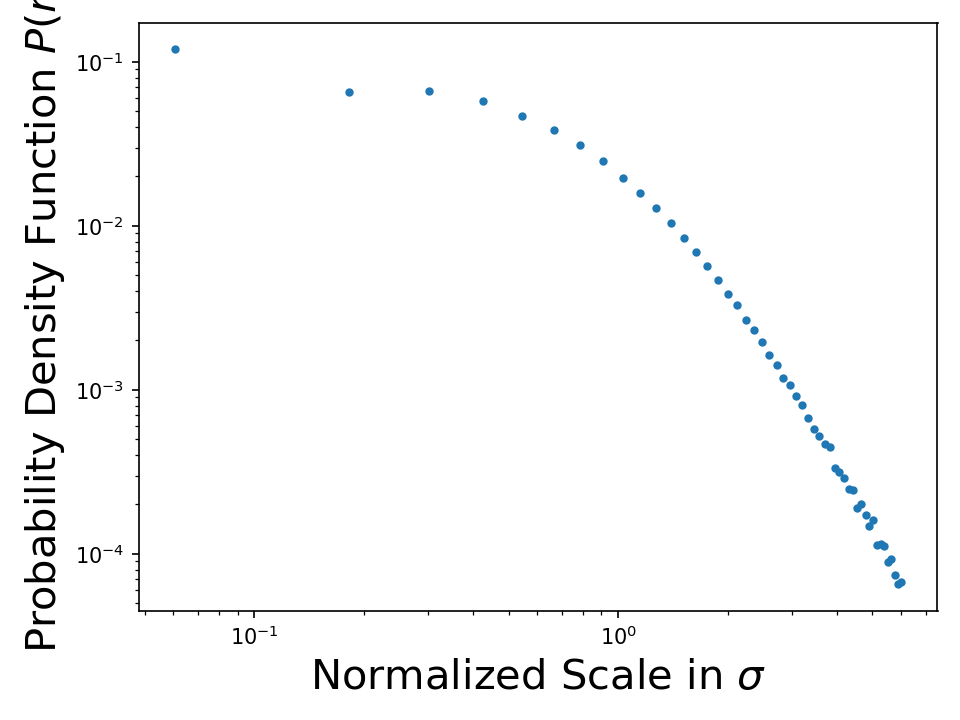
\includegraphics[width=\linewidth]{images/gen_dist_replication_returns_other_pos_log.png}
        \caption{Heavy-tail distribution}
        \label{fig:ref_distribution}
    \end{subfigure}
    \hfill
    \begin{subfigure}{0.32\textwidth}
        \centering
        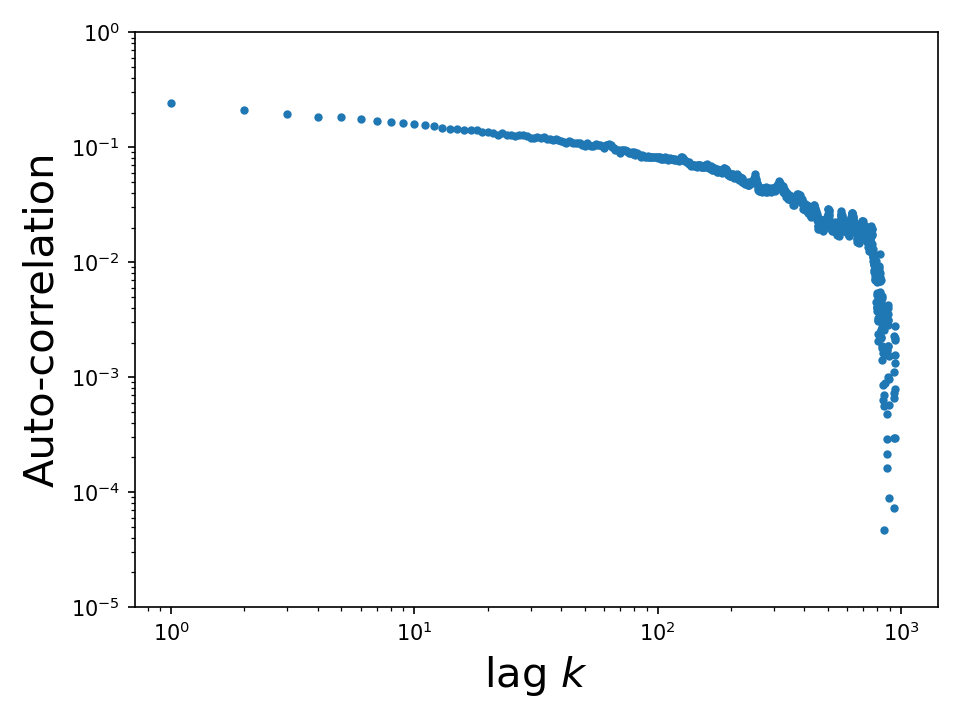
\includegraphics[width=\linewidth]{images/ref_vol_clus_replication_returns_other.png}
        \caption{Volatility clustering}
        \label{fig:ref_vol_clustering}
    \end{subfigure}
    \hfill
    \begin{subfigure}{0.32\textwidth}
        \centering
        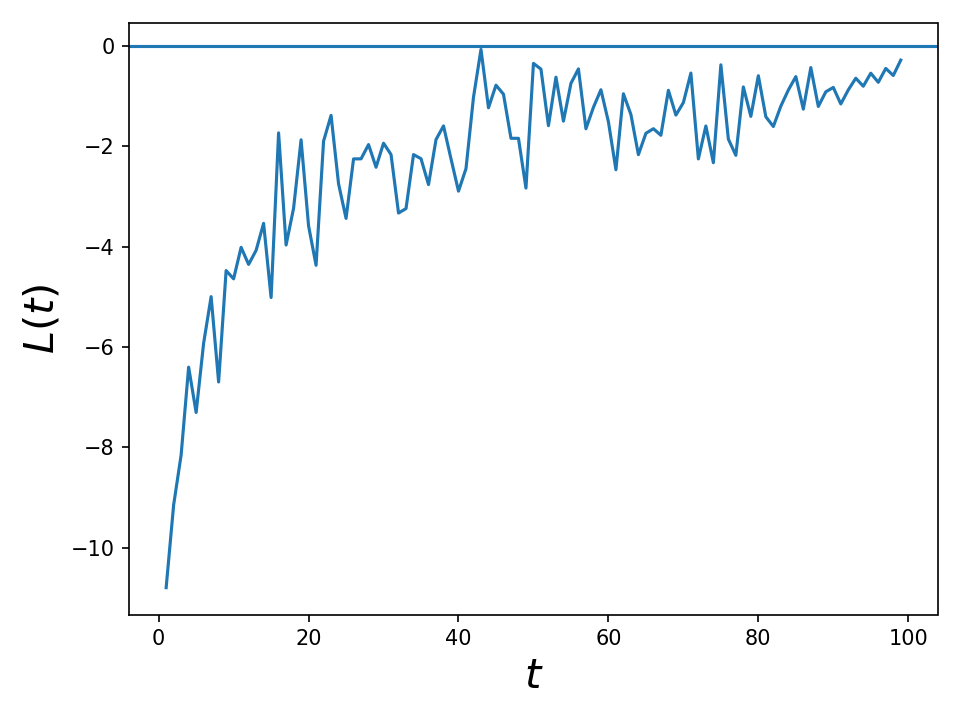
\includegraphics[width=\linewidth]{images/lev_eff_replication_returns_other.png}
        \caption{Leverage effect}
        \label{fig:ref_lev_eff}
    \end{subfigure}

    \caption{Stylized Facts for FTS, S\&P500 log-returns.}
    \label{fig:three_graphs}
\end{figure}

It is important to state that financial returns do not follow a Gaussian behavior, indeed large price fluctuations occur more frequently than under Brownian motion, breaking random walk assumption \cite{mandelbrot1963variation, fama1965random}. Moreover, the fact that returns have polynomial-like tail decay \cite{cont2001empirical} implies that, contrary to what was believed before \cite{mandelbrot1963variation}, they have finite variance, and often unstable of infinite fourth moment \cite{gopikrishnan1999scaling}. Therefore, it is modern consensus that returns are not necessarily symmetric Lévy-stable process \cite{mantegna1995scaling}, but that assuming a Gaussian tail distribution would significantly underestimate risk. 

\section{Classical Models}
\label{sec:classical_models_literature}
Classical FTS models often address the non-Gaussian behavior by extending upon the basic Brownian motion framework because of its favourable framework. In particular, GARCH-like models \cite{bollerslev1986generalized} focus on time-varying volatility, where by construction the model is conditionally heteroskedastic, meaning that large shocks are followed by higher volatility and period of calm by lower ones. Merton's jump diffusion \cite{merton1976option} instead build on the continuous Geometric Brownian Motion (GBM) by adding a Poisson jump component, the jumps. These are two common model to capture stylized facts about financial data, which is why they would work as baseline. 

In a GARCH(1,1) we have that the conditional variance behaves accordingly to:\(\sigma_t^2=\omega+\alpha\epsilon_{t-1}^2+\beta \sigma_{t-1}^2\), where \(\omega>0\) and \(\alpha, \beta \ge 0\), with a persistent condition \(\alpha+\beta<1\). Despite their parsimony, GARCH models remain a competitive benchmark in financial time-series modelling due to their interpretability, tractable likelihood, and well-known statistical properties. 

In order to understand Merton's model we have to introduce first the GBM. Given an asset price \(S_t\) it is said to follow a GBM if:
\begin{equation}
    \label{eq:blackscholes}
    dS_t=\mu S_td\tau+\nu S_tdW_t
\end{equation}
where \(\mu\) is the constant drift, \(\nu>0\) is the constant volatility, and \(W_t\) is a standard Brownian motion. The core feature of this process is the multiplicative structure of the noise term, which is scaled by price level. Applying Itô's Lemma to \(\log S_t\) it is possible to derive:
$$S_t=S_0\exp{\left[\left(\mu-\frac12\nu^2\right)\tau+\nu W_t\right]}$$
therefore with the GBM assumption, , Black and Scholes \cite{black1973pricing}, implied that log-returns are normally distributed over any interval, while heteroskedasticity is introduced in price space. Their model remain highly influencial even nowadays, nevertheless it has some fundamental limitations due to the inability of Gaussian's innovations to replicate the heavy tails, excess kurtosis, and sudden discontinuities exhibited by real returns. 

Merton addressed this by imposing a compounded Poisson jump process onto the GBM \cite{merton1976option}, yielding the model that takes his name:
$$dS_t=\mu S_tdt+\nu S_tdW_t+S_{t^-}(J-1)dP_t$$
where \(P_t\) is the Poisson process with intensity \(\lambda\) and J is a random jump multiplier \(J\sim \mathcal{N}(\mu_j, \sigma_J^2)\). This result in log-returns distribution that is a Poisson's weighted mixture of Gaussians. 

Both of these models impose parametric distributions, while this enable easier interpretation and a well understood behavior that makes them valuable baselines, it is also their limiting factor, that do not enable them to learn complex, highly dimensional joint distribution, and is also why they require re-fitting whenever their estimation regime changes.

\section{Deep Generative Models}
Deep generative models are non-parametric, therefore they learn implicitly the data distribution, \(p_{\text{data}(x)}\), and can theoretically learn all the stylized facts simultaneously, including temporal and feature dependencies. Before diffusion models, two families of models mostly dominated the FTS modeling and generation scene: GANs \cite{goodfellow2014generative, creswell2018generative,yoon2019time,vuletic2024fingan} and VAEs \cite{kingma2014auto, kingma2019introduction}. GANs, Generative Adversarial Networks, consist of a non-cooperative minmax game between a Generator \(G_\theta(z)\) and a Discriminator \(D_\phi(x)\): by learning implicitly the distribution without explicit likelihood constraints they are able to avoid over-smoothing and generate more sharp and diverse samples. On the other hand, GANs often suffer of mode collapse, when the Generator fail to capture fully the target distribution \(p_{\text{data}(x)}\), mapping only to few modes. Moreover, GANs suffer from training instability due to the non-convex nature of the minmax problem, which makes the optimization difficult.

VAEs, Variational Autoencoders, provide a probabilistic framework where input data \(x\) are mapped into a latent space through an encoder and reconstructed via a decoder \(p_\theta(x|z)\), with the system trained to maximise the Evidence Lower Bound (ELBO), fundamentally balancing a reconstruction term and a KL regularisation term. While theoretically sounding, VAEs suffer mainly from two limitations: posterior collapse and over-smoothing. The former, happens when the KL regularisation term dominates early training phases and push the approximate posterior towards the prior before any informative encoding is learned, degenerating into an unconditional mean model. The latter, because of the Gaussian decoder assumption, minimise square reconstruction error, which sistematically compress variance and suppress tail events. Both model families have limitations that make them difficult to apply to FTS. In contrast, diffusion models provide a probabilistic framework and a stable training objective, at the cost of slower sampling.

\section{Score-based Diffusion Models}
\label{sec:scorediffmodels}
Score-based diffusion models revolve around a simple idea: rather than learning to generate data directly, a model could learn to denoise it. If data are gradually corrupted, up to a point, where they become indistinguishable from a fixed prior, the generation is then reduced to learn how to reverse the corruption process, one step at the time. What makes the reversal possible is the score function,\(\nabla_x \log p(x)\), that intuitively points in the direction one should move a noisy sample to make it more likely under the current data distribution.

The score function is chosen to represent the probability distribution of the generative model, because it encodes the geometry of the distribution and it does not require the computation of the normalizing constant, $Z_\theta$, which are often complex and unstable. Therefore, our goal is to learn a function that can approximate the score, \(s_\theta(x)\approx\nabla_x \log p(x)\) by minimizing the Fisher divergence between \(\mathbb{E}_{p(x)}=\left[\|\nabla_x\log p(x)-s_\theta (x)\|^2_2\right]\) the two distributions. This can be achieved without knowing the ground truth through methods called score matching \cite{hyvarinen2005estimation, vincent2011connection}. 

Once we have trained a score-based model, we use Langevin dynamics \cite{parisi1981correlation} to draw samples from it. Due to the weighting of the Fisher Divergence the score estimate are only reliable in high density region, but Langevin dynamics must traverse low-density regions to move between modes, guided by the score. To address this, data are perturbated with a sequence of noise levels, \(\sigma_1< \sigma_2< \dots<\sigma_L\), that populate low-density regions and makes score estimation accurate everywhere. Therefore, we move to estimating a Noise-Conditional Score-based Network (NCSN) \cite{song2019generative}, \(s_\theta(x,i)\), where \(i=1,2,\dots,L\). The choosen noise is often Gaussian \(\mathcal{N}(0,\sigma_i^2I)\) and the sampling is performed through annealed Langevin dynamics. This model is often referred to as Score Matching with Langevin Dynamics (SMLD). 

Independently, DDPM's authors \cite{ho2020ddpm} reached a similar framework, where the forward process is not motivated through score estimation, but is a fixed Markov chain that gradually injects Gaussian noise into the data. With the advantage that the marginal distribution at any step \(t\) has a closed form:
$$q(x_t|x_{t-1})=\mathcal{N}\left(x_t;\sqrt{1-\beta_t}x_{t-1}, \beta_tI\right), \quad q(x_t|x_0)=\mathcal{N}\left(x_t;\sqrt{\bar{\alpha}}x_0, (1-\bar{\alpha})I\right)$$
where \(\alpha_t:=1-\beta_t\) and \(\bar{\alpha}_t:=\prod_{s=1}^t\alpha_t\) \cite{ho2020ddpm}. They also shows that by reparametrizing \(x_t(x_0,\epsilon)=\sqrt{\bar{\alpha_t}}x_0+\sqrt{1-\bar{\alpha_t}}\epsilon\), where \(\epsilon \sim \mathcal{N}(0,I)\), the objective function get simpliefied to a noise prediction loss:
\begin{equation}
\label{eq:ddpm_noise_loss}
\mathcal{L}=\mathbb{E}_{t,x_0,\epsilon}\left[\|\epsilon -\epsilon_\theta(\sqrt{\bar{\alpha_t}}x_0+\sqrt{1-\bar{\alpha_t}}\epsilon,t)\|\right]  
\end{equation}

The key connection that makes the score matching tractable is due to Vincent \cite{vincent2011connection}, who showed that the intractable Fisher Divergence over the clean distribution \(p(x)\) can be replaced by a noisy one \(q_\sigma(\tilde{x}|x)=\mathcal{N}\left(\tilde{x};x,\sigma^2I\right)\), yielding Denoising Score Matching (DSM) objective:
$$\mathcal{L}_{\text{DSM}}=\mathbb{E}_{x\sim p(x),\space \tilde{x}\sim q_\sigma(\tilde{x}|x)}\left[\|s_\theta(\tilde{x},\sigma)-\nabla_{\tilde{x}} \log q_\sigma(\tilde{x}|x)\| \right]$$Since \(q_\sigma(\tilde{x}|x)\) is Gaussian then it is fully tractable with \(\nabla_{\tilde{x}} \log q_\sigma(\tilde{x}|x)=-\epsilon/\sigma\), where \(\tilde{x}=x+\sigma\epsilon\) and \(\epsilon\sim\mathcal{N}(0,I)\) is the added noise. The score therefore points from the corrupted sample \(\tilde{x}\) back towards the clean data \(x\), scaled by \(\sigma^2\). This reveals that the DDPM noise-prediction objective (Eq.\ref{eq:ddpm_noise_loss}) 
is not conceptually different from score matching up to a scaling factor, since 
$\epsilon_\theta(x_t,t)\approx -\sqrt{1-\bar{\alpha_t}}s_\theta(x_t,t)$. By 
consequence, DDPM and NCSN can be understood as discrete instantiations of a more 
general principle: corrupting data with a noise process and learning to reverse it 
by estimating scores. When training over multiple noise levels, the DSM objective 
becomes a weighted sum:
$$
\mathcal{L}_{\text{NCSN}} = \sum_{i=1}^{L} \lambda(\sigma_i)\,
\mathbb{E}_{x\sim p(x),\,\tilde{x}\sim q_{\sigma_i}(\tilde{x}|x)}
\left[\left\|s_\theta(\tilde{x}, \sigma_i) - 
\nabla_{\tilde{x}}\log q_{\sigma_i}(\tilde{x}|x)\right\|^2\right]
$$
Since the score satisfies $\nabla_{\tilde{x}}\log q_{\sigma_i}(\tilde{x}|x) = 
-\epsilon/\sigma_i$, its magnitude varies strongly across noise levels, and the 
choice of weighting $\lambda(\sigma_i)$ is non-trivial. Song \cite{song2019generative} 
proposes $\lambda(\sigma_i) = \sigma_i^2$ to approximately equalise the contribution 
of each noise level, but this choice is heuristic rather than principled. 

% Song score funcitions
% Song score functions
\begin{figure}[htbp]
  \centering
  {\small
  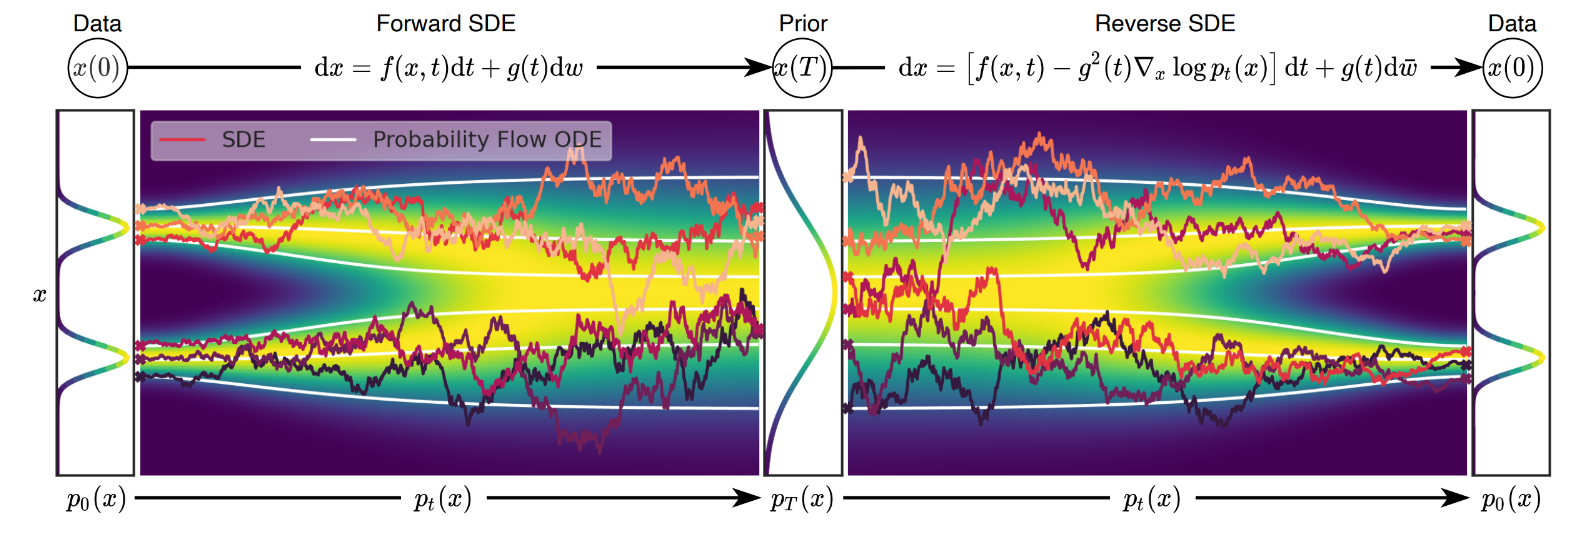
\includegraphics[width=\textwidth]{images/Overview_score_generative-modeling_Song.png}
  }
  \caption{Data can be mapped to a noise distribution (the prior) with an SDE (Eq.~\ref{eq:generalsde}), and reverse this SDE for generative modeling
(Eq.~\ref{eq:reverse_sde}). We can also reverse the associated probability flow ODE (Eq.~\ref{eq:probability_flow}), which yields a deterministic process that samples from the same distribution as the SDE. Both the reverse-time SDE and probability flow ODE can be obtained by estimating the score \(\nabla_x\log p_t(x_t)\). Source: Song et al.\ \cite{song2021score}.}
  \label{fig:sde_diffusion_process}
\end{figure}


Song \cite{song2021score} formalize the difusion model process by lifting DDPM and SMLD into a contiunous framework. He showed that the diffusion process \(\{x_t\}_{t=0}^T\) indexed by a continuous time variable \(t\in[0,T]\), where \(x_0\sim p_0\) is composed by i.i.d. samples of the dataset, and \(x_T\sim p_T\), for which we have a tractable form, can be modeled as the solution to an Itô SDE:
\begin{equation}
    \label{eq:generalsde}
    dx_t=f(x_t,t)dt+g(t)dW_t
\end{equation}
where \(W\) is the standard Wiener process, \(f(\cdot,t):\mathbb{R}^d\xrightarrow[]{}\mathbb{R}^d\) is a vector valued function called the drift coefficient of \(x_t\), and \(g(\cdot):\mathbb{R}\xrightarrow[]{}\mathbb{R}\) is a scalar function known as
the diffusion coefficient of \(x_t\). The SDE admits a unique strong solution provided the coefficients are globally Lipschitz \cite{oksendal2003stochastic}, and \(p_T\) is chosen to be a tractable prior, typically a Gaussian with fixed mean and variance, that contains no information about \(p_0\). 

The key insight is that the forward process admits a corresponding reverse-time SDE, in particular it has been shown \cite{anderson1982reversetime} that the reverse of a diffusion process is a diffusion process itself. By starting from samples \(x_T \sim p_T\) and reversing the process from \(t=T\) to \(t=0\), we can obtain samples \(x_0\sim p_0\) according to the relationship:
\begin{equation}
    \label{eq:reverse_sde}
    dx_t=\left[f(x_t, t)-g(t)^2\nabla_x\log p_t(x_t)\right]dt + g(t)d\bar{W}_t
\end{equation}

where \(\bar{W_t}\) is a standard Wiener process that flows back from \(T\) to \(0\). Since \(\nabla_x\log p_t(x_t)\) is unknown then we estimate it by using \(s_\theta(x_t,t)\). Importantly, Song et al. \cite{song2021score} showed that for any SDE (Eq.\ref{eq:generalsde}) there exists a corresponding deterministic Ordinary Differential Equation (ODE), called probability flow ODE, that produce the same family of marginal distributions \(\{p_t\}_{t\in[0,T]}\):
\begin{equation}
    \label{eq:probability_flow}
    dx_t=\left[f(x_t,t)-\frac12g(t)^2\nabla_x\log p_t(x_t)\right]dt
\end{equation}
substituting the intractable score with the learned one yields a Neural ODE, where given starting conditions $x_T\sim p_T$ we can deterministically sample to produce a sample from, approximately, \(p_0\). This sampling technique is possibly more efficient. 

Two specific SDE formulation that matched the SMLD and DDPM ones, in continuous time, hence when we assume that the number of noise steps \(N\xrightarrow[]{}\infty\), are: Variance Exploding (VE) and Variance Preserving (VP). The former sets \(f(\cdot,t)=0\) and is defined as:
\begin{equation}
    \label{eq:ve}
    dx_t=\sqrt{\frac{d[\sigma^2(t)]}{dt}}dW_t
\end{equation}
so that \(x_t=x_0+\sigma\epsilon\), where \(\epsilon\sim \mathcal{N}(0,I)\), therefore the marginal's variance grows unbounded as \(\sigma(t)\) increases. VP is instead:
$$dx_t=-\frac12 \beta(t)x_tdt+\sqrt{\beta(t)}dW_t$$
with drift \(f(x_t,t)=-\frac12\beta(t)x_t\) and \(g(t)=\sqrt{\beta(t)}\). This setting preserve unit variance when \(x_0\) has it as well with the marginal converging to \(\mathcal{N}(0,I)\) as \(t\xrightarrow[]{}T\).

The reverse SDE can be solved numerically through different samplers. 
Song \cite{song2021score} employs the Euler-Maruyama method, a first-order 
discretisation of the reverse-time SDE:
\begin{equation}
\label{eq:euler_maruyama}
x_{t+dt} \leftarrow x_t + \left[f(x_t,t) - g(t)^2 s_\theta(x_t,t)\right]|dt| 
+ g(t)\sqrt{|dt|}\,\epsilon, \quad \epsilon \sim \mathcal{N}(0,I)
\end{equation}
though any suitable numerical solver can in principle be substituted.

This continuous formulation has the advantage of decoupling the noise schedule 
from the choice of sampler, admitting common schedules such as linear, 
exponential, and cosine. However, both DDPM \cite{ho2020ddpm} and the SDE-based 
framework of Song \cite{song2021score} require hundreds of Neural Function 
Evaluations (NFEs) to produce a single sample, and neither provides a principled 
answer to how noise levels should be chosen, nor how network inputs and outputs 
should be scaled.

\section{Elucidating the Design Space of Diffusion Models (EDM)}
\label{sec:edm_literature}
Karras et al.\ \cite{karras2022elucidating} identify that prior formulations, including 
DDPM and Song's SDEs, choose in a dependable way four conceptually distinct design choices: the noise schedule, the parametrisation of network inputs and outputs, the weighting 
of the loss across noise levels, and the numerical solver used at sampling time. 
EDM separates these into four independent components and optimises each 
separately.

\textbf{Preconditioning} \quad EDM parametrises the denoiser as:
\begin{equation}
    \label{eq:edm_denoiser}
    D_\theta(x;\sigma) = c_{\text{skip}}(\sigma)\,x + 
    c_{\text{out}}(\sigma)\,F_\theta\!\left(c_{\text{in}}(\sigma)\,x;\, 
    c_{\text{noise}}(\sigma)\right)
\end{equation}
where $F_\theta$ is the raw neural network and 
$c_{\text{skip}}, c_{\text{out}}, c_{\text{in}}, c_{\text{noise}}$ are scalar 
functions of $\sigma$ chosen so that the inputs to $F_\theta$ have unit variance, 
the training targets have unit variance, and errors in $F_\theta$ are amplified as 
little as possible. For data with standard deviation $\sigma_{\text{data}}$, 
EDM sets:
$$
c_{\text{skip}}(\sigma)= \frac{\sigma_{\text{data}}^2}{\sigma^2 + 
    \sigma_{\text{data}}^2}, \quad 
    c_{\text{out}}(\sigma)= \frac{\sigma \cdot \sigma_{\text{data}}}
    {\sqrt{\sigma^2 + \sigma_{\text{data}}^2}}
$$
$$
c_{\text{in}}(\sigma)=\frac{1}{\sqrt{\sigma^2 + 
    \sigma_{\text{data}}^2}}, \quad
    c_{\text{noise}}(\sigma)=\frac{1}{4}\ln(\sigma)
$$
The skip connection $c_{\text{skip}}(\sigma)$ has a simpler interpretation: at low $\sigma$, $c_{\text{skip}} \to 1$ and the network mostly 
copies the input, a sensible prior when the noisy observation is already close to 
the data; at high $\sigma$, $c_{\text{skip}} \to 0$ and the network must 
reconstruct the clean signal from scratch. This mechanism helps stabilizing the training 
across the full noise range without requiring separate tuning for each noise level. 

\textbf{Loss weighting} \quad The EDM training objective is defined with respect to the denoiser 
$D_\theta(x;\sigma)$. Given a clean sample $x_0 \sim p_0$ and noise 
$\epsilon \sim \mathcal{N}(0, I)$, the noisy observation is 
$\tilde{x} = x_0 + \sigma\epsilon$, as in VE, and the loss is:
\begin{equation}
    \label{eq:edm_loss}
    \mathcal{L}_{\text{EDM}} = \mathbb{E}_{\sigma,\, x_0,\, \epsilon}
    \left[\lambda(\sigma)\,\left\|D_\theta(x_0 + \sigma\epsilon;\,\sigma) - 
    x_0\right\|^2\right]
\end{equation}
The effective weight for each sample on the raw network prediction $F_\theta$ is 
$\lambda(\sigma)\,c_{\text{out}}(\sigma)^2$. EDM sets 
$\lambda(\sigma) = c_{\text{out}}(\sigma)^{-2}$, which cancels out this factor and equalises loss contribution across all noise levels. Without this correction, high-noise steps would dominate the gradient signal, producing a model that denoises well at large $\sigma$ but fails to recover fine 
structure poorly, which is precisely the failure mode left unaddressed by NCSN. 

\textbf{Noise distribution} Rather than sampling $\sigma$ uniformly in $t$ as in DDPM, EDM concentrates training effort on the noise range that is most informative. At very low $\sigma$ the noisy input is nearly identical to the clean data, and at very 
high $\sigma$ the target collapses to the dataset mean. The informative region is in the middle, therefore EDM targets it by drawing:
\begin{equation}
    \label{eq:edm_sigma_sampling}
    \ln\sigma \sim \mathcal{N}(P_{\text{mean}},\, P_{\text{std}}^2)
\end{equation}
with defaults $P_{\text{mean}} = -1.2$ and $P_{\text{std}} = 1.2$, calibrated 
on ImageNet \cite{deng2009imagenet}. 

\begin{figure}[htbp]
  \centering
  {\small
  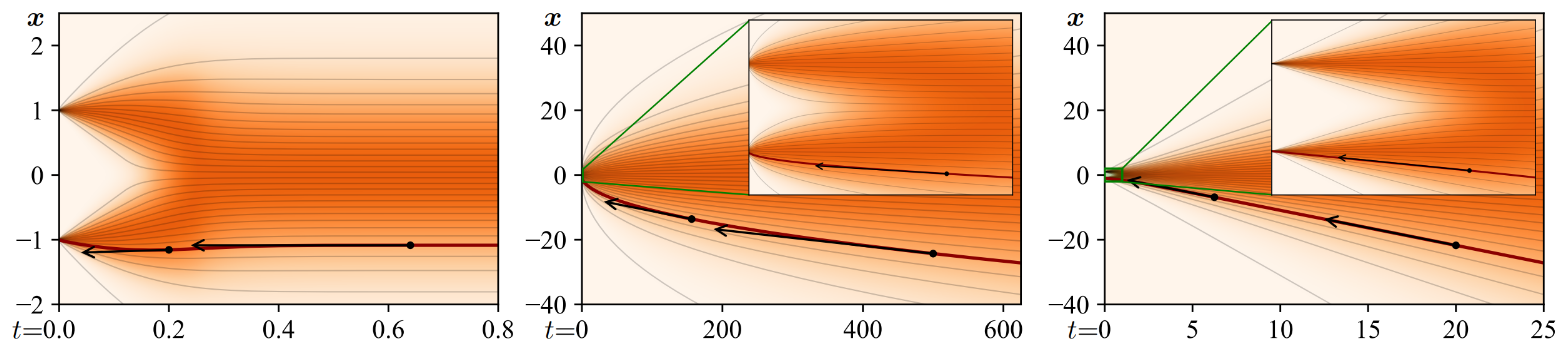
\includegraphics[width=\textwidth]{images/EDM_Sampler.png}
  }
  \caption{ A sketch of ODE curvature in 1D where \(p_{\text{data}}\) is two Dirac peaks at \(x\pm1\) Horizontal \(t\) axis is chosen to show \(\sigma\in[0,0.25]\) in each plot, with insets showing \(\sigma\in[0,1]\) near the data. Example local gradients are shown with black arrows. \emph{Left.} Variance preserving ODE of Song et al. \cite{song2021score} has
solution trajectories that flatten out to horizontal lines at large \(\sigma\). Local gradients start pointing towards data only at small \(\sigma\). \emph{Center.} Variance exploding variant has extreme curvature near data and the solution trajectories are curved everywhere. \emph{Right.} With the schedule used by DDIM \cite{song2021denoising} and us, as
\(\sigma\) increases the solution trajectories approach straight lines that point towards the mean of data. As \(\sigma \rightarrow 0\), the trajectories become linear and point towards the data manifold. Source: Karras et al.\ \cite{karras2022elucidating}.}
  \label{fig:karras_sampler_image}
\end{figure}

\textbf{Sampler design} \quad
At inference time, EDM employs a deterministic second-order Heun ODE solver with 
a $\rho$-power noise schedule:
\begin{equation}
    \label{eq:edm_sampler}
    \sigma_i = \left(\sigma_{\text{max}}^{1/\rho} + \frac{i}{N-1}
\left(\sigma_{\text{min}}^{1/\rho} - \sigma_{\text{max}}^{1/\rho}\right)
\right)^{\!\rho}, \quad i = 0, \dots, N-1
\end{equation}
with $\rho = 7$. The power-law schedule concentrates discretisation steps at
small $\sigma$, where the ODE curvature is highest and denoising errors have the
greatest impact on sample quality, which is why instead of \(\rho=3\) that equalize the truncation error at each step they chose higher values. This resulted in equivalent sample quality to DDPM with approximately $7\times$ fewer NFEs, and better convergence as shown in Fig.\ \ref{fig:karras_sampler_image}. Moreover, the sampler is independent of the training procedure, therefore a model trained with the EDM loss could be evaluated with any compatible ODE or SDE solver.

\textbf{Stochastic Heun Sampler} \label{sec:stochastic_heun} \quad Karras et al.\ also propose a stochastic variant of the Heun solver in which a controlled amount of noise is reinjected before each denoising step. Before applying the standard second-order Heun update, the current noise level $\sigma_i$ is temporarily inflated to
\begin{equation}
    \label{eq:stochastic_heun}
    \hat{\sigma}_i = \sigma_i\sqrt{1 + \gamma_i^2}, \qquad
    \gamma_i = \min\!\left(\frac{S_{\text{churn}}}{N},\;\sqrt{2}-1\right),
\end{equation}
and the sample is perturbed as $\hat{x}_i = x_i + \sqrt{\hat{\sigma}_i^2 - \sigma_i^2}\;\epsilon_i$ with $\epsilon_i \sim \mathcal{N}(0,I)$, before the Heun step proceeds from $(\hat{x}_i,\hat{\sigma}_i)$ to $\sigma_{i+1}$. The scalar $S_{\text{churn}} \geq 0$ is the sole stochasticity parameter: when $S_{\text{churn}} = 0$ every $\gamma_i = 0$ and the algorithm collapses to the deterministic ODE solver, while positive values allow the trajectory to briefly re-enter a higher-noise regime at each step, counteracting discretisation errors at the cost of additional noise injections.

\section{Conditional Score-Based Diffusion for Time Series (CSDI)}
\label{sec:csdi_literature}

Standard diffusion models, as described in the previous sections, learn to 
generate unconditionally from $p_{\text{data}}$. For time series imputation, or more generally for conditional generation, given a subset of conditioning observed values related to the target entries we can compute the conditional distribution $p(x^{\text{ta}} | x^{\text{co}})$. CSDI \cite{tashiro2021csdi} make this possible via a masking mechanism that is applied both at training and inference time. 

\textbf{Architectural lineage} \quad
To understand the architectural choices made in CSDI, it is useful to look at  
evolution of CSDI's backbone. PixelCNN \cite{oord2016pixel} established the core 
ideas of modeling high-dimensional data through local conditional information by using masked convolutions, residual connections, and gated activations, enabling the understanding of local and global relationships. WaveNet \cite{oord2016wavenet} transferred 
this logic from images to raw audio by replacing 2D masked image convolutions 
with 1D causal dilated convolutions, allowing the receptive field to grow exponentially with depth while maintaining causality. DiffWave 
\cite{kong2021diffwave} then kept the WaveNet-style residual architecture but abandoned the autoregressive component entirely, since it moves to a diffusion model. Because during denoising the target is the entire signal, future context is accessible to the model, and causal convolutions are replaced by bidirectional dilated convolutions. The key 
inherited components from WaveNet are the stacks of residual blocks, the diffusion-step conditioning, gated activations, and skip aggregation. CSDI \cite{tashiro2021csdi} then adapts this DiffWave backbone to multivariate 
time-series imputation, replacing the convolutional modeling with 
two-dimensional attention and introducing an explicit conditioning mechanism 
for observed values. The evolution therefore follows a clear progression: firstly autoregressive local dependency modelling, secondly dilated temporal convolutions, thirdly  diffusion denoising with WaveNet-style residual blocks, and then CSDI's conditional time-series denoiser with attention. 

% CSDI high-level overview
\begin{figure}[htbp]
  \centering
  {\small
  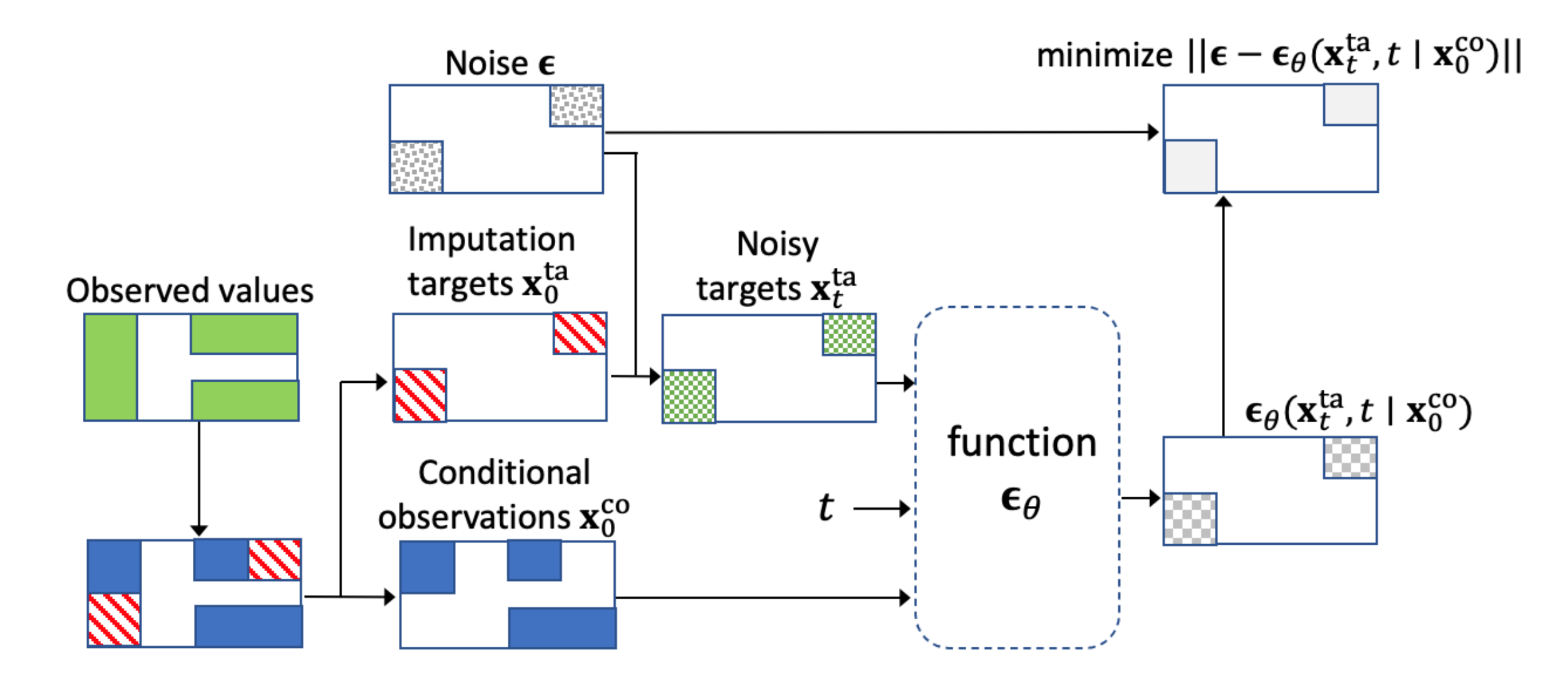
\includegraphics[width=\textwidth]{images/CSDI_high_level_overview.png}
  }
  \caption{The self-supervised training procedure of CSDI for implementation of time series imputation. The colored areas in each rectangle represent the existence of values. The green and white areas represent observed and missing values, respectively, and white areas are padded with zeros to fix the shape of the inputs. Zero padding is also applied to all white areas. As with Figure 2, the observed values are separated into red imputation targets \(x_0^{\text{ta}}\) and blue conditional observations \(x_0^{\text{co}}\). For the extended targets \(\hat{x}_0^{\text{ta}}\), the area of value 0 shows dummy values. Source: CSDI\ \cite{tashiro2021csdi}.}
  \label{fig:csdi_high_level}
\end{figure}

\textbf{Conditional denoising mechanism} \quad At each denoising step $t$, the CSDI model takes as input three quantities: 
the noisy target $x^{\text{ta}}_t$, which gets zero-padded at conditioning indices; the 
clean conditioning observations $x^{\text{co}}_0$, which gets zero-padded at target indices; and a binary mask $m^{\text{co}} \in \{0,1\}^{K \times L}$ indicating which entries are observed, where $K$ is the number of channels and $L$ is the sequence length. The conditional score network is therefore 
$\epsilon_\theta(x^{\text{ta}}_t, t \mid x^{\text{co}}_0, m^{\text{co}})$, and 
the training objective is:
\begin{equation}
\label{eq:csdi_objective}
    \min_\theta\; \mathbb{E}\left[\left\|\epsilon - 
    \epsilon_\theta\!\left(x^{\text{ta}}_t, t \;\middle|\; 
    x^{\text{co}}_0, m^{\text{co}}\right)\right\|^2_{m^{\text{ta}}}\right]
\end{equation}
where $\|\cdot\|^2_{m^{\text{ta}}}$ denotes that the squared error is evaluated 
only at target indices. The conditioning information $x^{\text{co}}_0$ and 
$m^{\text{co}}$ are kept fixed throughout the reverse process, while only the 
target entries are denoised. 

% CSDI high-level overview
\begin{figure}[htbp]
  \centering
  {\small
  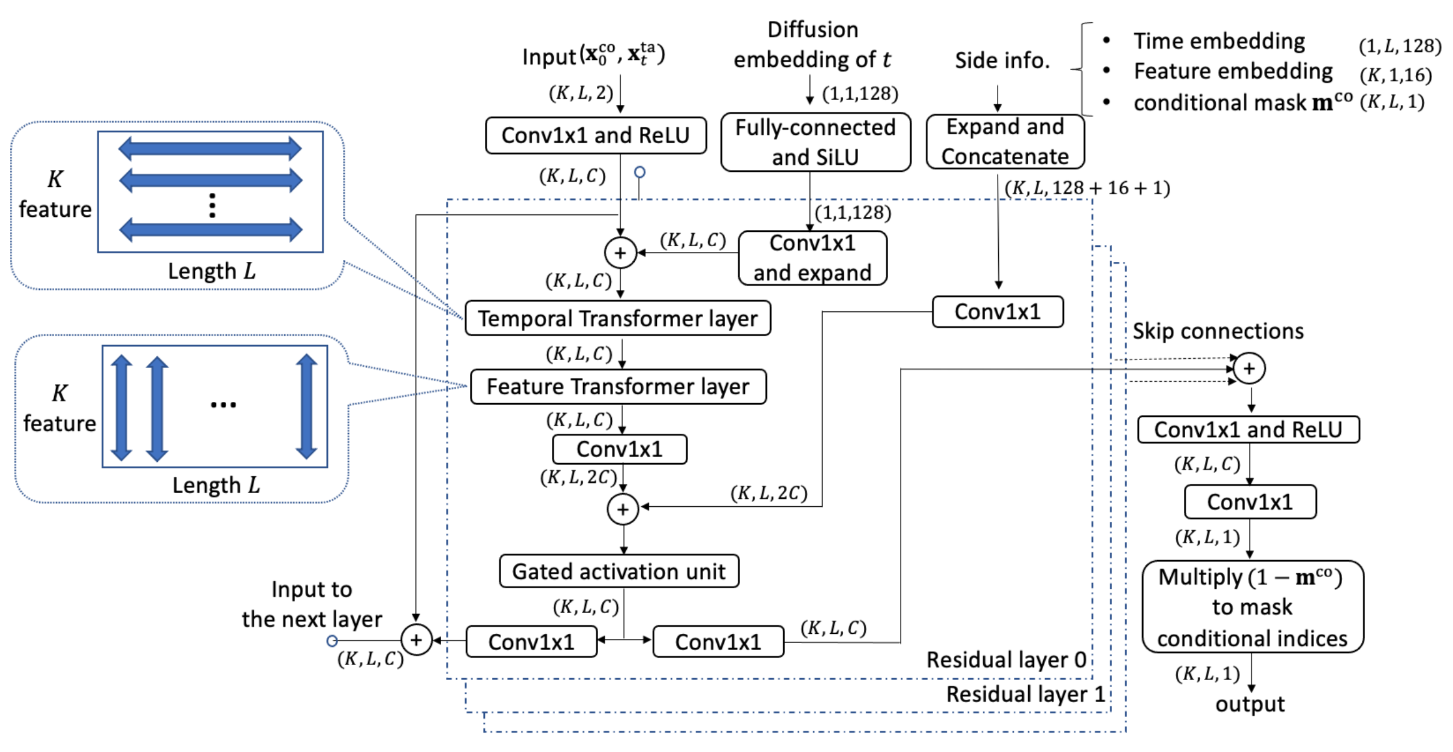
\includegraphics[width=\textwidth]{images/CSDI_architecture_full.png}
  }
  \caption{Architecture of \(\epsilon_\theta\) in CSDI for multivariate time series imputation. Source: CSDI\ \cite{tashiro2021csdi}.}
  \label{fig:csdi_high_level}
\end{figure}

\textbf{2D attention over time and features} \quad The central innovation of CSDI over DiffWave is the replacement of dilated 
temporal convolutions with a two-dimensional attention mechanism. Two Transformer 
layers \cite{vaswani2017attention} operate in sequence within each residual block: a temporal Transformer which operates along the time axis, capturing short- and long-range temporal dependencies within each channel, and a feature Transformer operating along the channel axis, capturing cross-channel dependencies between variables. This 2D attention allows the model to learn both the temporal dynamics of each channel and the 
contemporaneous relationships between channels, without the quadratic cost of 
attending jointly over the full time-feature product space. The overall block 
structure residual connections, skip aggregation, and gated activations 
is inherited directly from DiffWave and ultimately from WaveNet. 

\textbf{Positional and diffusion-step embeddings} \quad Three types of embeddings are added to the latent representation to allow the model to simultaneously distinguish temporal position, noise level, and channel 
identity: a sinusoidal diffusion-step embedding encoding the current noise level 
$t$; a temporal embedding encoding absolute position along the time axis; and a 
feature embedding encoding the identity of each channel. The diffusion-step 
embedding plays the same role as the noise conditioning $c_{\text{noise}}(\sigma)$ 
in the EDM preconditioning, ensuring that the denoiser is aware of the current noise level. 

\textbf{Self-supervised training strategy and limitations} \quad CSDI introduces several masking strategies for training (random, historical, 
mixed, and test-pattern) that simulate different conditioning and target splits 
during training, effectively providing a sort of data augmentation through varied 
masking.

\section{GBM--style SDE}
\label{sec:gbm_sde_ch2}
The idea of using CSDI for FTS modeling was explored previously by Gihum Kim et al. in \emph{A diffusion-based generative model for financial time series via geometric Brownian motion} \cite{kim2025diffusion}. While interesting this work lack the details needed in order to be replicable and provide ambiguous statements about what is actually persue. 

They showed that starting from the Black--Scholes equation (Eq.~\ref{eq:blackscholes}) and 
applying It\^{o}'s lemma to \(X_t = \log S_t\), one obtains:
\[
    dX_t = \left(\mu_t - \frac{1}{2}\nu_t^2\right)dt + \nu_t\,dW_t,
\]
where \(\nu_t > 0\) is the instantaneous volatility. Choosing 
\(\mu_t = \frac{1}{2}\nu_t^2\) cancels the drift term, yielding a 
VE-type SDE in log-price space (Eq.~\ref{eq:ve}), with the forward 
process reduced to:
\begin{equation}
    \label{eq:forward_ve}
    x_t = x_0 + \sigma\epsilon, \quad \epsilon \sim \mathcal{N}(0, I),
\end{equation}
where \(\sigma\) denotes the noise level at diffusion step \(t\), 
distinct from the instantaneous volatility. 

It is important to stress that this drift cancellation is a deliberate 
modelling choice, not a consequence of the GBM dynamics: the resulting 
process is no longer a pure GBM but rather a VE-type diffusion in 
log-price space inspired by it. The financial interpretation is that, 
while noise remains additive in log-price space, the exponential map back to price space induces effective heteroskedasticity with volatility that scales with the price level.

However, an ambiguity in the original paper requires clarification. In Section 3.1, 'Geometric Brownian motion in score-based Models' is stated:
\begin{quote}
    \emph{[...] the GBM-based formulation naturally injects larger noise into higher--value regimes, thereby preserving economically meaningful dynamics in the generated trajectories. It inherently scales noise with the underlying price level, enhancing the model’s sensitivity to large market movements. As a result, the diffusion process can more accurately capture stylized facts such as volatility clustering and heavy tails.}
\end{quote}
Nevertheless, in Section 3.1.2, the authors state:
\begin{quote}
    \emph{For each selected stock, we calculated daily log-returns, defined 
    as \(r_t = \log(p_t / p_{t-1})\), where \(p_t\) represents the 
    adjusted closing price on day \(t\). To create training samples 
    suitable for diffusion modeling, we applied a sliding window approach 
    to the log-return sequences.}
\end{quote}
This indicates that the model is trained on log-returns, not on log-prices. 
Log-prices \(X_t = \log S_t\) are non-stationary, making them undesirable 
as direct training targets. The GBM-style diffusion derivation above 
operates on log-prices in theory, but practical training on log-returns.

\section{Heavy--Tailed Diffusion Models}

A natural question follows from the heavy--tailed nature of financial time series: if the target distribution exhibits rare but economically important extreme events, should the forward perturbation process also be heavy--tailed, so that both the noised data and the terminal prior better reflect the structure of the underlying data structure.

This question remains open in literature, but in order to narrow down the problem we should consider the following points:
\begin{itemize}
    \item Can a diffusion model based on Gaussian perturbations learn a heavy--tailed target distribution at all?
    \item If it can, how much modelling capacity should be explicitly allocated to tail behaviour rather than to the bulk of the distribution?
\end{itemize}
Recent theoretical work suggests that Gaussian perturbations are not automatically invalid in the presence of heavy tails. Yu et al.\ \cite{yu2026diffusion} study standard Gaussian score-based diffusion models when the target distribution is heavy--tailed. Under a tractable kernel-based score estimator, they derive minimax guarantees showing a distinction between tail regimes: for exponentially decaying tails, Gaussian diffusion remains statistically robust, while for polynomially decaying tails the score-estimation and sampling rates depend explicitly on the tail index. Since financial log-returns are commonly modelled as having polynomial-like tail decay, this result is directly relevant to financial time series. It does not imply that Gaussian diffusion is unusable, but it does indicate that heavy tails increase the statistical difficulty of score learning. 

A complementary line of work modifies the perturbation distribution itself. Pandey et al.\ \cite{pandey2024heavytailed} propose heavy--tailed diffusion models based on multivariate Student-\(t\) perturbation kernels, leading to \(t\)-EDM. In this framework, the degrees-of-freedom parameter \(\nu\) controls tail heaviness: smaller values of \(\nu\) produce heavier tails, while the Gaussian case is recovered in the limit \(\nu \to \infty\). Because the Kullback--Leibler divergence between Student-\(t\) distributions does not generally admit a convenient closed form, they replace the usual KL-based objective with a \(\gamma\)-power divergence. This objective is not an ELBO in the standard sense, but it recovers the KL divergence in the appropriate limited regime. 

A more radical alternative is to replace Brownian motion itself with a heavy--tailed jump process. Yoon et al.\ \cite{yoon2023score} propose the L\'evy-It\^o Model, which uses isotropic \(\alpha\)-stable L\'evy processes instead of Brownian motion. They derive the corresponding reverse-time SDE and train the model through fractional denoising score matching. Such an approach is conceptually appealing for financial data, where jumps and rare events are structurally important. However, it requires a different and specific score object and reverse process, as well as a substantially different mathematical framework from the Gaussian EDM--CSDI model used in this work. This does not gurantee the same freedom for design choices as EDM.

Consequently, this thesis study a Gaussian EDM--CSDI baseline for conditional financial time-series generation, with explicit tail-sensitive evaluation. Heavy--tailed perturbation kernels and L\'evy-driven score models may improve tail fidelity, but they also introduce additional modelling choices and may alter the trade-off between tail accuracy, bulk distributional fit, training stability, and computational simplicity.
% \section{Summary}

% This chapter has established the theoretical foundations upon which the present work is built. We began by characterising financial time series through their core stylized facts and discussed the related challenges with modeling such properties. Subsequently, we presented the classical approaches GARCH and Merton's jump diffusion, along with their ability to capture some of these features through parametric assumptions, and their structural limitations. 

% Deep generative models lift this restriction, but GANs and VAEs introduce their own pathologies, in particular mode collapse and over-smoothing, respectively, that are particularly damaging in the heavy-tailed, asymmetric setting such as financial returns. Score-based diffusion models offer a more principled alternative: a stable training objective grounded in denoising score matching, a well-understood probabilistic framework, and the flexibility to condition generation on partial observations. 

% Within this family, the EDM framework of Karras et al.\cite{karras2022elucidating} provides a structured decomposition of the design space by using preconditioning, loss weighting, noise distribution, and sampler, that resolves several heuristic choices left open by DDPM and Song et al. \cite{ho2020ddpm, song2021score}. CSDI \cite{tashiro2021csdi} then introduces the conditional masking mechanism and the factored two-dimensional attention architecture that make conditional generation over multivariate time series more feasible. Together, these two frameworks form the direct theoretical basis of this thesis, which combines EDM preconditioning and loss weighting with a CSDI-style backbone to generate conditional values. 

% A prior attempt to unify these ideas in a financial setting was made by Kim et al.\cite{kim2025diffusion}, who derived a VE-type forward process from GBM dynamics by cancelling the drift term in log-price space and applying CSDI as the backbone. While conceptually motivated, the paper contains reproducibility limitations and a notable internal inconsistency: the theoretical derivation operates on log-prices, yet the reported experiments train on log-returns. Furthermore, claims that the GBM formulation inherently captures volatility clustering and heavy tails are overstated: once the model is trained on log-returns rather than log-prices, the price-level scaling that motivates those claims no longer applies directly to the training signal. The present work takes this prior contribution as context and background, adopts the same CSDI backbone, but replaces the VE-style SDE formulation with the EDM framework, which offers a more principled and flexible treatment of the noise schedule, preconditioning, and loss weighting.